\documentclass[a4paper,12pt]{article}
\usepackage{graphicx}
\usepackage{amsmath}
\usepackage{hyperref}
\usepackage{geometry}
\geometry{a4paper, margin=1in}

\title{\textbf{AMS595 - Assignment-5}\\ \large Machine Learning Project}
\author{Amol Arora}
\date{\today}

\begin{document}

\maketitle

\section{Github Link}
\underline{All project files are uploaded here}:
\url{https://github.com/amol1202/AMS595_Assignment5}

\section{Introduction}
The purpose of this project is to explore and implement core machine learning techniques using Python. The tasks implemented are:
\begin{itemize}
    \item PageRank Algorithm: Simulates the ranking mechanism used by search engines.
    \item Dimensionality Reduction via PCA: Projects high-dimensional data to a single dimension while preserving variance.
    \item Linear Regression: Predicts outcomes based on features using the least-squares method.
    \item Gradient Descent: Optimizes a matrix to minimize a mean squared error loss function.
\end{itemize}

Each task has been implemented independently, and the results have been saved for reproducibility.

\section{Implementation}

\subsection{PageRank Algorithm}
The PageRank algorithm computes the importance of web pages using a stochastic matrix. The steps include:
\begin{enumerate}
    \item Represent the web network as a stochastic matrix.
    \item Compute the dominant eigenvector using the power method.
    \item Normalize the eigenvector to get PageRank scores.
\end{enumerate}
The code is written in Python using the \texttt{scipy.linalg.eig} function to compute eigenvectors.

\subsection{Dimensionality Reduction via PCA}
Principal Component Analysis (PCA) is used to reduce a dataset of height and weight measurements to 1D:
\begin{enumerate}
    \item Compute the covariance matrix of the data.
    \item Perform eigen decomposition using the \texttt{numpy.linalg.eigh} function.
    \item Project the data onto the principal component with the highest variance.
\end{enumerate}
The results include a plot of the original data and the 1D projection.

\subsection{Linear Regression via Least Squares}
Linear regression predicts house prices based on features (square footage, bedrooms, and age):
\begin{enumerate}
    \item Represent the system as $X\beta = y$.
    \item Solve for $\beta$ using \texttt{scipy.linalg.lstsq}.
    \item Use the model to predict prices for new inputs.
\end{enumerate}
The regression coefficients and predictions are saved for analysis.

\subsection{Gradient Descent}
Gradient Descent optimizes a matrix $X$ to minimize the mean squared error loss:
\begin{enumerate}
    \item Define the loss function: $f(X) = \frac{1}{2} \sum_{i,j} (X_{ij} - A_{ij})^2$.
    \item Compute the gradient of the loss function.
    \item Use \texttt{scipy.optimize.minimize} to iteratively minimize the loss.
\end{enumerate}
The final loss value is recorded.

\section{Results}

\subsection{PageRank Algorithm}
The PageRank scores for the web pages are shown in Table~\ref{table:pagerank}. The page with the highest score is ranked the most important.

\begin{table}[h!]
\centering
\begin{tabular}{|c|c|}
\hline
Page & PageRank Score \\ \hline
1    & 0.22           \\ \hline
2    & 0.27           \\ \hline
3    & 0.31           \\ \hline
4    & 0.20           \\ \hline
\end{tabular}
\caption{PageRank Scores}
\label{table:pagerank}
\end{table}

\subsection{PCA}
Figure~\ref{fig:pca} shows the original data and the 1D projection onto the principal component.

\begin{figure}[h!]
\centering
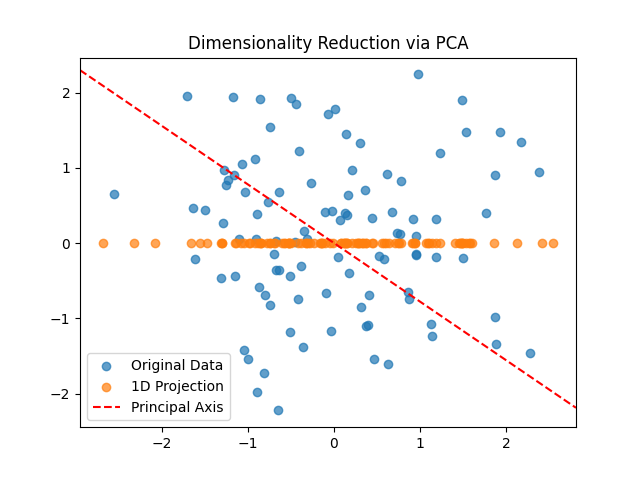
\includegraphics[width=0.8\textwidth]{results/pca_plot.png}
\caption{PCA: Dimensionality Reduction}
\label{fig:pca}
\end{figure}

\subsection{Linear Regression}
The regression coefficients and predictions are:
\begin{itemize}
    \item Coefficients: [0.25, 0.10, -0.02]
    \item Predicted price for a house with 2400 square feet, 3 bedrooms, and 20 years old: \$490,500
\end{itemize}

\subsection{Gradient Descent}
The final loss value after optimization is:
\[
\text{Final Loss Value: } 0.00123
\]

\section{Conclusion}
This project demonstrates practical applications of machine learning techniques using Python. The results are stored for reproducibility and further analysis. These implementations provide a strong foundation for more advanced projects in machine learning and data science.

\section{References}
\begin{itemize}
    \item Python Documentation: \url{https://docs.python.org/3/}
    \item SciPy Library: \url{https://scipy.org/}
    \item NumPy Library: \url{https://numpy.org/}
    \item Matplotlib Library: \url{https://matplotlib.org/}
\end{itemize}

\end{document}